\chapter{Categories and Fundamental Examples}
\label{CatFundamentals} % Always give a unique label
% use \chaptermark{}
% to alter or adjust the chapter heading in the running head

\section{Category Definitions}

\begin{definition}
    A \Emph{category} $\catname{C}$ is given by the following data: \begin{enumerate}
        \item a class $\catname{Ob}(\catname{C})$ of objects of $\catname{C}$
        \item a family $\Hom_{\catname{C}}$ associating with each pair $A, B \in \catname{C}$ a class $\Hom_{\catname{C}}(A,B)$ of morphisms from $A$ to $B$
    \end{enumerate}
    so that:
    \begin{enumerate}
        \item For a morphism $f \in \Hom_{\catname{C}}(A,B)$, we say that $A$ is the \Emph{domain} object of $f$ and \Emph{codomain} object of $f$, and we write $f:A\rightarrow B$. 
        \item For each object $A$ of $\catname{C}$ there is a designated \Emph{identity morphism} $\id_A \in \Hom_{\catname{C}}(A,A)$ (i.e. $\id_A:A\rightarrow A$).
        \item For all $A, B, C \in \catname{Ob}(\catname{C})$ a mapping \begin{equation*}
                \circ: \Hom_{\catname{C}}(B,C)\times \Hom_{\catname{C}}(A,B) \rightarrow \Hom_{\catname{C}}(A,C)
        \end{equation*}
            called composition exists, and is defined such that for all $f \in \Hom_{\catname{C}}(A,B)$ and $g \in \Hom_{\catname{C}}(B,C)$, the following diagram commutes:
				\begin{center}
					\begin{tikzpicture}[baseline= (a).base]
						\node[scale=1] (a) at (0,0){
						  \begin{tikzcd}
						  		& B \ar[dr, "g"] & \\
                    			A \ar[ur, "f"] \ar[rr, "g\circ f"] & & C
						  \end{tikzcd}
						};
					\end{tikzpicture}
				\end{center} 
                such that $g\circ f \in \Hom_{\catname{C}}(A,C)$ is called the \Emph{composite morphism}.
    \end{enumerate}
    This data is subject to the following axioms: \begin{enumerate}
        \item For any objects $A$ and $B$ and morphism $f:A\rightarrow B$, the composites $\id_B\circ f$ and $f\circ \id_A$ are equal to $f$.
        \item For any composable triple of morphisms $f:A\rightarrow B$, $g:B\rightarrow C$, and $h:C\rightarrow D$, the composites $h\circ(g\circ f)$ and $(h\circ g)\circ f$ are equal. In particular, the following diagram commutes:
            \begin{center}
               \tikzset{every picture/.style={line width=0.75pt}} %set default line width to 0.75pt        

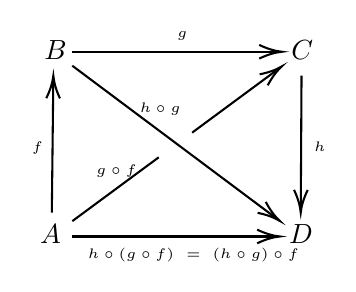
\begin{tikzpicture}[x=0.75pt,y=0.75pt,yscale=-1,xscale=1]
%uncomment if require: \path (0,300); %set diagram left start at 0, and has height of 300


% Text Node
\draw (125,142.4) node [anchor=north west][inner sep=0.75pt]    {$A$};
% Text Node
\draw (127,53.4) node [anchor=north west][inner sep=0.75pt]    {$B$};
% Text Node
\draw (246,53.4) node [anchor=north west][inner sep=0.75pt]    {$C$};
% Text Node
\draw (245,142.4) node [anchor=north west][inner sep=0.75pt]    {$D$};
% Text Node
\draw (121,102.4) node [anchor=north west][inner sep=0.75pt]  [font=\tiny]  {$f$};
% Text Node
\draw (191,49.4) node [anchor=north west][inner sep=0.75pt]  [font=\tiny]  {$g$};
% Text Node
\draw (257,102.4) node [anchor=north west][inner sep=0.75pt]  [font=\tiny]  {$h$};
% Text Node
\draw (173,83.4) node [anchor=north west][inner sep=0.75pt]  [font=\tiny]  {$h\circ g$};
% Text Node
\draw (152,113.4) node [anchor=north west][inner sep=0.75pt]  [font=\tiny]  {$g\circ f$};
% Text Node
\draw (148,153.4) node [anchor=north west][inner sep=0.75pt]  [font=\tiny]  {$h\circ ( g\circ f) \ =\ ( h\circ g) \circ f$};
% Connection
\draw    (132.13,138) -- (132.85,74) ;
\draw [shift={(132.87,72)}, rotate = 450.64] [color={rgb, 255:red, 0; green, 0; blue, 0 }  ][line width=0.75]    (10.93,-3.29) .. controls (6.95,-1.4) and (3.31,-0.3) .. (0,0) .. controls (3.31,0.3) and (6.95,1.4) .. (10.93,3.29)   ;
% Connection
\draw    (142,60.5) -- (241,60.5) ;
\draw [shift={(243,60.5)}, rotate = 180] [color={rgb, 255:red, 0; green, 0; blue, 0 }  ][line width=0.75]    (10.93,-3.29) .. controls (6.95,-1.4) and (3.31,-0.3) .. (0,0) .. controls (3.31,0.3) and (6.95,1.4) .. (10.93,3.29)   ;
% Connection
\draw    (252.44,72) -- (252.08,136) ;
\draw [shift={(252.06,138)}, rotate = 270.32] [color={rgb, 255:red, 0; green, 0; blue, 0 }  ][line width=0.75]    (10.93,-3.29) .. controls (6.95,-1.4) and (3.31,-0.3) .. (0,0) .. controls (3.31,0.3) and (6.95,1.4) .. (10.93,3.29)   ;
% Connection
\draw    (142,142.11) -- (183.65,111.35)(199.74,99.47) -- (241.39,68.7) ;
\draw [shift={(243,67.52)}, rotate = 503.55] [color={rgb, 255:red, 0; green, 0; blue, 0 }  ][line width=0.75]    (10.93,-3.29) .. controls (6.95,-1.4) and (3.31,-0.3) .. (0,0) .. controls (3.31,0.3) and (6.95,1.4) .. (10.93,3.29)   ;
% Connection
\draw    (142,67.23) -- (240.4,140.82) ;
\draw [shift={(242,142.02)}, rotate = 216.79] [color={rgb, 255:red, 0; green, 0; blue, 0 }  ][line width=0.75]    (10.93,-3.29) .. controls (6.95,-1.4) and (3.31,-0.3) .. (0,0) .. controls (3.31,0.3) and (6.95,1.4) .. (10.93,3.29)   ;
% Connection
\draw    (142,149.5) -- (240,149.5) ;
\draw [shift={(242,149.5)}, rotate = 180] [color={rgb, 255:red, 0; green, 0; blue, 0 }  ][line width=0.75]    (10.93,-3.29) .. controls (6.95,-1.4) and (3.31,-0.3) .. (0,0) .. controls (3.31,0.3) and (6.95,1.4) .. (10.93,3.29)   ;

\end{tikzpicture} 
            \end{center}
    \end{enumerate}
    That is, the composition law is associative and unital with the identity morphisms serving as two-sided identites.
\end{definition}

\begin{remark}
    The objects of a category are in bijective correspondence with the identity morphisms, which are uniquely determined by the property that they serve as two-sided identities with composition. Thus, we can define a category as a collection of morphisms with a partially defined composition operation that has certain special morphisms which are used to recognize composable pairs and which serve as two-sided identites. 
\end{remark}


\begin{example}
    \leavevmode
    \begin{enumerate}
        \item $\Set$ is the category with sets as its objections and set-theoretic functions, with specified domain and codomain, as its morphisms
        \item $\Topp$ is the category with topological spaces as its objects and continuous functions as its morphisms.
        \item $\Set_*$ ($\Topp_*$) are the categories with sets (spaces) with a specified basepoint as objects and basepoint preserving (continuous) functions as morphisms. Note that a \Emph{basepoint} is a distinguished point in the set (space).
        \item $\Grp$ is the category with groups homomorphisms as morphisms. The categories $\Ring$ of associative and unital rings and ring homomorphisms and $\catname{Field}$ of fields and field homomorphisms are defined similarly.
        \item For a fixed unital but not necessarily commutative ring $R$, $\Rmod$ is the category of left $R$-modules and $R$-module homomorphisms. Th:is category is denoted by $\Vect$ when the ring happends to be a field $k$ and abbreviated as $\catname{Ab}$ (for abelian groups) in the case of $\catname{Mod}_{\Z}$, as a $\Z$-module is precisely an abelian group.
        \item $\catname{Graph}$ is the category with graphs as objects and graph morphisms (functions carrying vertices to vertices and edges to edges, preserving incidence relations) as morphisms. In the variant $\catname{DirGraph}$, objects are directed graphs, whose edges are now depicted as arrows, and morphisms are directed graph morphisms, which preserve sources and targets.
        \item $\catname{Man}$ is the category with smooth (i.e. infinitely differentiable) manifolds as objects and smooth maps as morphisms.
        \item $\catname{Meas}$ is the category with measurable spaces as objects and measurable functions as morphisms. 
        \item $\catname{Poset}$ is the category with partially ordered sets as objects and order-preserving functions as morphisms.
        \item $\catname{Ch}_R$ is the category with chain complexes of $R$-modules as objects and chain homomorphisms as morphisms.
            \begin{definition}
                A \Emph{chain complex} $C_*$ is a collection $(C_n)_{n \in \Z}$ of $R$-modules equipped with $R$-module homomorphisms $d:C_n\rightarrow C_{n-1}$, called \Emph{boundary homomorphisms}, with the property that $d^2 = 0$, i.e., the composite of any two boundary maps is the zero homomorphism. A map of chain complexes $f:C_* \rightarrow C_*'$ is comprised of a collection of homomorphisms $f_n:C_n\rightarrow C_n'$ so that $df_n = f_{n-1}d$ for all $n \in \Z$.
            \end{definition}
        \item For any \Emph{signature} $\sigma$, specifying $n$-array relation symbols, and for any collection of well formed sentences $\mathbb{T}$ in the first order language associated to $\sigma$, there is a category $\catname{Model}_{\mathbb{T}}$ whose objects are $\sigma$-structures that \Emph{model} $\mathbb{T}$, i.e., sets equipped with appropriate $n$-array relations satisfying the axioms $\mathbb{T}$. Morphisms are functions that preserve the specified $n$-array relations in the ``usual sense." (4-6, 9, 10 are special cases of this)
    \end{enumerate}
\end{example}

These are all examples of \Emph{concrete} categories, those whose objects have underlying sets and whose morphisms are functions between those underlying sets.

\begin{example}
    \leavevmode
    \begin{enumerate}
        \item For a unital ring $R$, $\catname{Mat}_R$ is the category whose objects are positive integers and in which the set of morphisms from $n$ to $m$ is the set $m\times n$ with values in $R$. Composition is by matrix multiplication \begin{equation*}
                n\xrightarrow{A}m,\;\;m\xrightarrow{B}k,\;\;\;\rightsquigarrow\;\;\;n\xrightarrow{B\cdot A}k
        \end{equation*}
            with identity matrices serving as the identity morphisms.
        \item A group $G$ (or, more generally, a monoid) defines a category $\catname{B}G$ with a single object. The group elements are its morphisms, each group element representing a distinct endomorphism of the single object, with composition given by multiplication. The identity element $e \in G$ acts as the identity morphism for the unique object in this category. Example \begin{equation*}
                \catname{B}S_3 = \begin{tikzcd} 
                    \text{\textperiodcentered} \ar[out = 215, in = 145, loop, distance=3em, "e"] \ar[out =125, in = 55, loop,distance=3em, "(12)"] \ar[out = 35, in = -35,  loop,distance=3em,"(23)"] \ar[out = 305, in = 235, loop, distance=3em,"(123)"] \ar[out = 80, in = 10, loop,distance=3em, "(13)"] \ar[out = 260, in = 190, loop,distance=3em, "(132)"] 
                \end{tikzcd}
            \end{equation*}
        \item A poset $(P,\leq)$ (or, more generally, a preorder) may be regarded as a category. THe elements of $P$ are the objects of the category and there exists a unieq morphism $x\rightarrow y$ if and only if $x \leq y$. Transitivity of the relation ``$\leq$" implies that the required composite morphisms exist. Reflexitivity implies that identity morphisms exist.
        \item For any ordinal $\alpha = \{\beta\vert\beta <\alpha\}$ defines a category whose objects are the smaller ordinals. For example, $\mathbf{O}$ is the category with no objects and no morphisms. $\mathbf{1}$ is the category with a single object and only its identity morphism. $\mathbf{2}$ is the category with two objects and a single non-identity morphism, conventionally depicted as $0\rightarrow 1$, $\mathbf{\omega}$ is the category \Emph{freely generated by the graph} \begin{equation*}
                0\rightarrow 1\rightarrow 2\rightarrow \hdots
        \end{equation*}
            in the sense that every non-identity morphism can be uniquely factored as a composite of morphisms in the displayed graph.
        \item A set may be regarded as a category in which the elements of the set define the objects and the only morphisms are the required identities. A category is \Emph{discrete} if every morphism is an identity.
        \item $\catname{Htpy}$ is the category with spaces as its objects and homotopy classes of continuous maps as its morphisms. 
        \item $\catname{Measure}$ has measure spaces as objects. One reasonable choice for the morphisms is to take equivalence classes of measurable functions, where a parallel pair of functions are equivalent if their domain of difference is contained within a set of measure zero.
    \end{enumerate}
\end{example}


\begin{definition}
    A category is \Emph{small} if it has only a set's worth of arrows.
\end{definition}

\begin{corollary}
    By our previous remark we have that a small category has only a set's worth of objects. If $\catname{C}$ is a small category, then there are functions \begin{equation*}
        \Hom_{\catname{C}}\;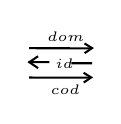
\begin{tikzpicture}[x=0.75pt,y=1.0pt,yscale=-1,xscale=1, baseline=(id.base)]
%uncomment if require: \path (0,300); %set diagram left start at 0, and has height of 300

%Straight Lines [id:da2656795330357933] 
\draw    (160.4,85.64) -- (150.4,85.63) ;
%Straight Lines [id:da0646642801892674] 
\draw    (139.8,85.21) -- (129.8,85.19) ;
\draw   (134.3,87.4) -- (130.1,85.24) -- (134.3,83.1) ;
%Straight Lines [id:da620246038923298] 
\draw    (159.49,90.84) -- (129.99,90.79) ;
\draw   (156.25,89.08) -- (159.89,90.75) -- (156.33,92.58) ;
%Straight Lines [id:da10731411804107904] 
\draw    (159.51,80.24) -- (130.01,80.19) ;
\draw   (156.67,78.48) -- (160.31,80.15) -- (156.75,81.98) ;

% Text Node
\draw (141.18,82.87) node(id) [anchor=north west][inner sep=0.75pt]  [font=\tiny,rotate=-359.44]  {$id$};
% Text Node
\draw (137.3,73.15) node [anchor=north west][inner sep=0.75pt]  [font=\tiny]  {$dom$};
% Text Node
\draw (138.9,92.15) node [anchor=north west][inner sep=0.75pt]  [font=\tiny]  {$cod$};


\end{tikzpicture}\;\catname{Ob}_{\catname{C}}
\end{equation*}
	that send a morphism to its domain and its codomain and an object to its identity.
\end{corollary}


\begin{definition}
    A category is \Emph{locally small} if between any pair of objects there is only a set's worth of morphisms. It is traditional to write $\catname{C}(X,Y)$ or $\Hom(X,Y)$ for the set of morphisms from $X$ to $Y$ in a locally small category $\catname{C}$. The set of arrows between a pair of fixed objects in a locally small category is typically called a \Emph{hom-set}.
\end{definition}


\begin{definition}
    An \Emph{isomorphism} in a category is a morphism $f:X\rightarrow Y$ for which there exists a morphism $g:Y\rightarrow X$ such that $g\circ f = \id_X$ and $f\circ g = \id_Y$. The objects $X$ and $Y$ are said to be \Emph{isomorphic} whenever there exists an isomorphism between $X$ and $Y$, in which case one writes $X\cong Y$.
\end{definition}

\begin{definition}
    An \Emph{endomorphism}, i.e., a morphism whose domain equals its codomain, that is an isomorphism is called an \Emph{automorphism}.
\end{definition}


\begin{example}
    \leavevmode
    \begin{enumerate}
        \item The isomorphisms in $\Set$ are precisely the \Emph{bijections}.
        \item The isomorphisms in $\Grp, \Ring, \catname{Field}$, or $\catname{Mod}_R$ are the bijective homomorphisms.
        \item The isomorphisms in the category $\Topp$ are the \Emph{homeomorphisms}, i.e., the continuosus functions with continuous inverse, which is a stronger property than merely being a bijective continuous function.
        \item The isomorphisms in the category $\catname{Htpy}$ are the \Emph{homotopy equivalences}
        \item In a poset $(P,\leq)$, the axiom of antisymmetry asserts that $x\leq y$ and $y\leq x$ imply that $x = y$. That is, the only isomorphisms in the category $(P,\leq)$ are identities.
    \end{enumerate}
\end{example}

\begin{question}
    In a concrete category, when are the isomorphisms precisely those maps in the category that induce bijections between the underlying sets? This requires some more constructions before we can answer it sufficiently.
\end{question}

\begin{definition}
    A \Emph{groupoid} is a category in whcih every morphism is an isomorphism.
\end{definition}

\begin{definition}
    \leavevmode
    \begin{enumerate}
        \item A \Emph{group} is a groupoid with one object.
        \item For any space $X$, its \Emph{fundamental groupoid} $\prod_1(X)$ is a category whose objects are the points of $X$ and whose morhpisms are endpoint-preserving homotopy classes of paths.
    \end{enumerate}
\end{definition}

\begin{definition}
    A \Emph{subcategory} $\catname{D}$ of a category $\catname{C}$ is defined by restricting to a subcollection of objects and subcollection of morphisms subject to the requirements that the subcategory $\catname{D}$ contains the domain and codomain of any morphism in $\catname{D}$, the identity morphism of any object in $\catname{D}$, and the composite of any composable pair of morphisms in $\catname{D}$.
\end{definition}


\begin{lemma}
    Any category $\catname{C}$ contains a \Emph{maximal groupoid}, the subcategory containing all of the objects and only those morphisms that are isomorphisms.
\end{lemma}
\begin{proof}
    Let $\catname{G}$ be the collection of isomorphisms with all objects in $\catname{C}$. First, since $\catname{G}$ contains all objects of $\catname{C}$, it contains all domains and codomains for its morphisms. Next, observe that for any object $X$ of $\catname{G}$, $\id_X\circ \id_X = \id_X$, so $\id_X$ is an isomorphism by definition, and is consequently in $\catname{G}$. Finally, let $f:A\rightarrow B$ and $g:B\rightarrow C$ be isomorphisms in $\catname{G}$ with inverse morphisms $f^{-1}:B\rightarrow A$ and $g^{-1}:C\rightarrow B$ (which are also in $\catname{G}$). Then, we consider the composite morphisms $g\circ f:A\rightarrow C$ and $f^{-1}\circ g^{-1}:c\rightarrow A$. It follows that \begin{equation*}
        (f^{-1}\circ g^{-1})\circ(g\circ f) = f^{-1}\circ g^{-1}\circ g\circ f = f^{-1}\circ \id_B\circ f = f^{-1}\circ f = \id_A
    \end{equation*}
    and \begin{equation*}
        (g\circ f)\circ (f^{-1}\circ g^{-1}) = g\circ f\circ f^{-1}\circ g^{-1} = g\circ \id_B\circ g^{-1} = g\circ g^{-1} = \id_C
    \end{equation*}
    so by definition we have that $g\circ f$ and $f^{-1}\circ g^{-1}$ are isomorphisms, and hence in $\catname{G}$. Thus $\catname{G}$ is a subcategory in $\catname{C}$. Moreover, every isomorphism of $\catname{C}$ is in $\catname{G}$, so it is indeed the \Emph{maximal groupoid} of $\catname{C}$.
\end{proof}


\begin{definition}
    For any category $\catname{C}$ and object $c$ of $\catname{C}$: \begin{enumerate}
        \item There is a category $c/\catname{C}$ whose objects are morphisms $f:c\rightarrow x$ with domain $c$ in which a morphism from $f:c\rightarrow x$ to $g:c\rightarrow y$ is a map $h:x\rightarrow y$ (in $\catname{C}$) between the codomains so that the triangle: 
            \begin{center}
                \begin{tikzpicture}[baseline= (a).base]
                    \node[scale=1] (a) at (0,0){
                      \begin{tikzcd}
                          & c \ar[dr, "g"] \ar[dl, swap, "f"] & \\
                            x \ar[rr, swap, "h"]  & & y
                      \end{tikzcd}
                    };
                \end{tikzpicture}
            \end{center} 
            \Emph{commutes}, i.e., so that $g= h\circ f$. This category is called the \Emph{slice category of $\catname{C}$ under $c$}.
        \item There is a category $\catname{C}/c$ whose objects are morphisms $f:x\rightarrow c$ with codomain $c$ in which a morphism from $f:x\rightarrow c$ to $g:y\rightarrow c$ is a map $h:x\rightarrow y$ (in $\catname{C}$) between the domains so that the triangle: 
            \begin{center}
                \begin{tikzpicture}[baseline= (a).base]
                    \node[scale=1] (a) at (0,0){
                      \begin{tikzcd}
                            x \ar[dr, swap, "f"] \ar[rr, "h"]  & & y\ar[dl, "g"] \\
                            & c & 
                      \end{tikzcd}
                    };
                \end{tikzpicture}
            \end{center} 
            \Emph{commutes}, i.e., so that $f= g\circ h$. This category is called the \Emph{slice category of $\catname{C}$ over $c$}.
    \end{enumerate}
\end{definition}


\section{Duality}

Let us consider the notion of ``reversing the arrows" of a particular category.

\begin{definition}
    Let $\catname{C}$ be any category. The \Emph{opposite category} $\catname{C}^{op}$ has \begin{enumerate}
        \item the same objects as in $\catname{C}$, and 
        \item a morphism $f^{op}$ in $\catname{C}^{op}$ for each morphism $f$ in $\catname{C}$ such that the domain of $f^{op}$ is defined to be the codomain of $f$ and the codomain of $f^{op}$ is defined to be the domain of $f$: that is \begin{equation*}
                f^{op}:X\rightarrow Y \in \catname{C}^{op} \;\;\leftrightsquigarrow\;\;f:Y\rightarrow X\in\catname{C}
        \end{equation*}
    \end{enumerate}
    That is, $\catname{C}^{op}$ has the same objects and morphisms as $\catname{C}$, except that ``each morphism is pointing in the opposite direction." THe remaining structure of the category $\catname{C}^{op}$ is given as follows: \begin{enumerate}
        \item For each object $X$, the arrow $\id_X^{op}$ serves as its identity in $\catname{C}^{op}$
        \item To define composition, observe that a pair of morphisms $f^{op}, g^{op}$ in $\catname{C}^{op}$ is composable precisely when the pair $g,f$ is composable in $\catname{C}$, i.e., precisely when the codomain of $g$ equals the domain of $f$. We then define $g^{op}\circ f^{op}$ to be $(f\circ g)^{op}$: 
            \begin{center}
                \begin{tikzpicture}[baseline= (a).base]
                    \node[scale=1] (a) at (0,0){
                      \begin{tikzcd}
                          f^{op}:X\rightarrow Y,g^{op}:Y\rightarrow Z \in \catname{C}^{op} \ar[r, rightsquigarrow] \ar[d, leftrightsquigarrow] & g^{op}\circ f^{op}:X\rightarrow Z\in\catname{C}^{op} \ar[d, leftrightsquigarrow] \\
                          g:Z\rightarrow Y,f:Y\rightarrow X \in \catname{C} \ar[r, rightsquigarrow] & f\circ g:Z\rightarrow X \in \catname{C}
                      \end{tikzcd}
                    };
                \end{tikzpicture}
            \end{center} 
    \end{enumerate}
\end{definition}

\begin{example}
    \leavevmode
    \begin{enumerate}
        \item $\catname{Mat}_R^{op}$ is the category whose objects are non-zero natural numbers and in which a morphism from $m$ to $n$ is an $m\times n$ matrix with values in $R$. 
        \item When a preorder $(P,\leq)$ is regarded as a category, its opposite category is the category that has a morphism $x\rightarrow y$ if and only if $y \leq x$. For example, $\mathbf{\omega}^{op}$ is the category freely generated by the graph \begin{equation*}
                \hdots \rightarrow 3\rightarrow 2\rightarrow 1\rightarrow 0.
        \end{equation*}
    \item If $G$ is a group, regarded as a one-object groupoid, the category $(\catname{B}G)^{op} \cong \catname{B}(G^{op})$ is again a one-object groupoid, and hence a group. The group $G^{op}$ is called the \Emph{opposite group} and is used to define right actions as a special case of left actions.
    \end{enumerate}
\end{example}

\begin{remark}
    Any theorem containing a universal quantification of the form ``for all categories $\catname{C}$" also necessarily applies to the opposites of these categories. Interpreting the result in the dual context leads to a \Emph{dual theorem}, proven by the dual of the original proof, in which the direction of each arrow appearing in the argument is reversed.
\end{remark}

\begin{lemma}
    The following are equivalent: \begin{enumerate}
        \item $f:x\rightarrow y$ is an isomorphism in $\catname{C}$
        \item For all objects $c \in \catname{C}$, post-composition with $f$ defines a bijection \begin{equation*}
                f_*:\catname{C}(c,x)\rightarrow \catname{C}(c,y)
        \end{equation*}
    \item For all objects $c \in \catname{C}$, pre-composition with $f$ defines a bijection \begin{equation*}
            f^*:\catname{C}(y,x)\rightarrow \catname{C}(x,c)
    \end{equation*}
    \end{enumerate}
    The is to say, isomorphisms in a locally small category are defined representably in terms of isomorphisms in the category of sets. However, this also applies to non-locally small categories given certain set theoretical foundations.
\end{lemma}
\begin{proof}
    First we will prove the equivalence $1. \iff 2.$:

    Assuming 1., namely that $f:x\rightarrow y$ is an isomorphism with inverse $g:y\rightarrow x$, then, as an immediate application of the associativity and identity laws for composition in a category, post-composition with $g$ defines an inverse function \begin{equation*}
        g_*:\catname{C}(c,y)\rightarrow \catname{C}(c,x)
    \end{equation*}
    to $f_*$ in the sense that the composites \begin{equation*}
        g_*\circ f_*:\catname{C}(c,x)\rightarrow \catname{C}(c,x)\;\;\text{and}\;\;f_*\circ g_*:\catname{C}(c,y)\rightarrow \catname{C}(c,y)
    \end{equation*}
    are both the identity function: for any $h:c\rightarrow x$ and $k:c\rightarrow y$, $g_*\circ f_*(h) = g\circ f\circ h = h$, and $f_*\circ g_*(k) = f\circ g \circ k = k$.

    Conversely, assuming 2., there must be an element $g \in \catname{C}(y,x)$ whose image under $f_*:\catname{C}(y,x)\rightarrow \catname{C}(y,y)$ is $\id_y$. By construction, $\id_y = f\circ g$. But, now by associativity of composition, the elments $g\circ f, \id_x \in \catname{C}(x,x)$ have the common image $f$ under the function $f_*:\catname{C}(x,x)\rightarrow \catname{C}(x,y)$, whence $g\circ f = \id_x$. Thus, $f$ and $g$ are inverse isomorphisms.

    To prove the equivalence $1.\iff 3.$ for all categories, we use the principle of duality. Indeed, since we have proven $1.\iff 2.$ for all categories, it applies to the category $\catname{C}^{op}$: i.e., a morphism $f^{op}:y\rightarrow x$ in $\catname{C}^{op}$ is an isomorphism if and only if \begin{equation*}
        f_*^{op}:\catname{C}^{op}(c,y)\rightarrow \catname{C}^{op}(c,x)
    \end{equation*}
    is an isomorphism for all $c \in \catname{C}^{op}$. Interpreting the data of $\catname{C}^{op}$ in its opposite category, the previous statement expresses the same mathematical content as \begin{equation*}
        f^*:\catname{C}(y,c)\rightarrow\catname{C}(x,c)
    \end{equation*}
    is an isomorphism for all $c \in \catname{C}$. That is: $\catname{C}^{op}(c,x) = \catname{C}(x,c)$, post composition with $f^{op}$ in $\catname{C}^{op}$ translates to pre-composition with $f$ in the opposite category $\catname{C}$. The notion of isomorphism is self-dual: $f^{op}:y\rightarrow x$ is an isomorphism in $\catname{C}^{op}$ if and only if $f:x\rightarrow y$ is an isomorphism in $\catname{C}$. So the equivalence $1.\iff 2.$ in $\catname{C}^{op}$ expresses the equivalence $1.\iff 3.$ in $\catname{C}$.
\end{proof}

\begin{definition}
    A morphism $f:x\rightarrow y$ in a category is \begin{enumerate}
        \item a \Emph{monomorphism} if for any parallel morphisms \begin{tikzcd} h,k:w \ar[r, shift left] \ar[r, shift right] & x \end{tikzcd}, $f\circ h = f\circ k$ implies that $h = k$ (left cancellable); or
        \item an \Emph{epimorphism} if for any parallel morphisms \begin{tikzcd} h,k:y \ar[r, shift left] \ar[r, shift right] & z \end{tikzcd}, $h\circ f = k\circ f$ implies that $h = k$ (right cancellable)
    \end{enumerate}
\end{definition}

\begin{remark}
    Note that a monomorphism or epimorphism in $\catname{C}$ is, respectively, an epimorphism or monomorphism in $\catname{C}^{op}$.
\end{remark}

\begin{note}
    In adjectival form, a monomorphism is \Emph{monic}, or in shorthand \Emph{mono}, and is denoted by ``$\rightarrowtail$," whil a epimorphism is \Emph{epic}, or in shortand \Emph{epi}, and is denoted by ``$\twoheadrightarrow$."
\end{note}

\begin{definition}[Alternative Mono and Epi Definitions]
    A morphism $f:x\rightarrow y$:\begin{enumerate}
        \item is a monomorphism in $\catname{C}$ if and only if for all objects $c \in \catname{C}$, post-composition with $f$ defines an injection $f_*:\catname{C}(c,x)\rightarrow \catname{C}(c,y)$.
        \item is an epimorphism in $\catname{C}$ if and only if for all objects $c \in \catname{C}$, pre-composition with $f$ defines an injection $f^*:\catname{C}(y,c)\rightarrow \catname{C}(x,c)$.
    \end{enumerate}
\end{definition}

\begin{example}
    Suppose $f:X\rightarrow Y$ is a monomorphism in the category of sets. Then in particular, given any two maps \begin{tikzcd}x,x':\mathbf{1} \ar[r, shift left] \ar[r,shift right] & X\end{tikzcd}, whose domain is the singleton set, if $f\circ x = f\circ x'$ then $x = x'$. Thus, monomorphisms are injective functions. Conversely, any injective function can easily be seen to be a monomorphism.


    Similarly, a function $f:X\rightarrow Y$ is an epimorphism in the category of sets if and only if it is surjective. Given functions \begin{tikzcd} h,k:Y\ar[r,shift left]\ar[r,shift right] & Z\end{tikzcd}, the equation $h\circ f = k\circ f$ says exactly that $h$ is equal to $k$ on the image of $f$. This implies that $h = k$ in the case where the image is all of $Y$.
\end{example}

\begin{example}
    Suppose that $x\xrightarrow{s}y\xrightarrow{r}x$ are morphisms so that $r\circ s = \id_x$. The map $s$ is a \Emph{section} or \Emph{right inverse} to $r$, while the map $r$ defines a \Emph{retraction} or \Emph{left inverse} to $s$. The maps $s$ and $r$ express the object $x$ as a \Emph{retract} of the object $y$.

    In this case, $s$ is always a monomorphism and, dually, $r$ is always an epimorphism. To acknowledge these one-sided inverses, $s$ is said to be a \Emph{split monomorphism} and $r$ is said to be a \Emph{split epimorphism}.
\end{example}

\begin{lemma}
    \leavevmode
    \begin{enumerate}
        \item[(i)] If $f:x\rightarrowtail y$ and $g:y\rightarrowtail z$ are monomorphisms, then so is $g\circ f:x\rightarrowtail z$.
        \item[(ii)] If $f:x\rightarrow y$ and $g:y\rightarrow z$ are morphisms so that $g\circ f$ is monic, then $f$ is monic.
    \end{enumerate}
    Dually: \begin{enumerate}
        \item[(i')] If $fLx\twoheadrightarrow y$ and $g:y\twoheadrightarrow z$ are epimorphisms, then so is $g\circ f: x\twoheadrightarrow z$.
        \item[(ii')] If $f:x\rightarrow y$ and $g:y\rightarrow z$ are morphisms so that $g\circ f$ is epic, then $g$ is epic.
    \end{enumerate}
\end{lemma}
